%\documentstyle[amssymb,12pt,draft,epsf,palatino]{nature-pvd}
\documentclass{natureprintstyle}
\bibliographystyle{naturemag}

\usepackage{aas_macros}

\usepackage{epsfig,caption}
\usepackage{color}
\usepackage{bm}
\usepackage{graphicx}
\usepackage{longtable}
% \usepackage{amssymb}
\usepackage{rotating,xcolor}
\usepackage{hyperref}
% \usepackage{tgbonum}

\usepackage{fontspec}
\setmainfont{texgyrepagella}[
  Extension = .otf,
  UprightFont = *-regular,
  BoldFont = *-bold,
  ItalicFont = *-italic,
  BoldItalicFont = *-bolditalic,
]

\usepackage[misc]{ifsym}

\title{Stellar Bars in Isolated Gas-Rich Galaxies Do Not Slow Down}

\author{Angus Beane$^{1*}$, Lars Hernquist$^1$, Elena D'Onghia$^{2,3}$, et al.}


\begin{document}

\maketitle

\let\thefootnote\relax\footnote{

\begin{affiliations}
\item Center for Astrophysics $|$ Harvard \& Smithsonian,  Cambridge, MA, USA

\item Department of Physics, University of Wisconsin-Madison, Madison, WI, USA

\item Department of Astronomy, University of Wisconsin-Madison, Madison, WI, USA

$^{*}$ \texttt{\mbox{angus.beane@cfa.harvard.edu}}

\end{affiliations}
}

\vspace{-3.5mm}
\begin{abstract}
  
  Elongated bar-like features are ubiquitous, occuring at the centres of
  approximately two-thirds of spiral disk galaxies \cite{2000AJ....119..536E,
  2007ApJ...657..790M}. Due to gravitational interactions between the bar and
  the other components of galaxies, it is expected that angular momentum and
  matter will redistribute between galactic components over long (Gyr)
  timescales in galaxies hosting a bar \cite{1972MNRAS.157....1L,
  1984MNRAS.209..729T, 1985MNRAS.213..451W}. Previous work has overwhelmingly
  provided the expectation that, due to these interactions, the bar pattern
  will slow its rotation over time \cite{1992ApJ...400...80H,
  2000ApJ...543..704D, 2002MNRAS.330...35A, 2002ApJ...569L..83A,
  2003MNRAS.341.1179A, 2003MNRAS.346..251O, 2005MNRAS.363..991H,
  2006ApJ...637..214M, 2007MNRAS.375..460W, 2009ApJ...697..293D}. We have
  performed a simulation of an isolated galactic disk hosting a strong bar
  which includes a state-of-the-art model of the interstellar medium. Here we
  show that in this simulation the bar pattern does not slow down over time,
  and instead remains at a stable, constant rate of rotation. This behavior
  has been observed in previous simulations but its explanation has remained
  elusive.\cite{1993AA...268...65F, 2010ApJ...719.1470V}. We propose an
  equilibrium mechanism which is consistent with our simulations. This result
  challenges our expectations for how barred galaxies redistribute angular
  momentum and matter over Gyr timescales, which is especially relevant for
  our understanding of how the Milky Way arrived at its present day state.
  
\end{abstract}

\vspace{1cm}

%%%%%%%%%%%%%%%%%%%%%%%%%%%%%%%%%%%%%%%%%%%%%%%%%%%%%


We have performed a simulation of a disk galaxy using the finite-volume
gravity-hydrodynamics code AREPO \cite{2010MNRAS.401..791S}. In AREPO, the
fluid is discretized as a moving Voronoi mesh. We use the additional physics
in the galaxy formation module Stars and MUltiphase Gas in GaLaxiEs (SMUGGLE)
\cite{2019MNRAS.489.4233M}. SMUGGLE is a comprehensive and self-consistent
galaxy formation model with a wide range of physical processes, including
radiative heating/cooling, star formation, and stellar feedback. More detailed
information on SMUGGLE is given in the Methods section.

Our disk galaxy is a modified version of the GALAKOS
model\cite{2020ApJ...890..117D}, which consists of a radially exponential and
vertically isothermal stellar disk along with a
Hernquist\cite{1990ApJ...356..359H} dark matter halo and bulge. After
$\sim2.5\,\textrm{Gyr}$ of evolution, the GALAKOS disk forms a bar consistent
with the Milky Way bar in terms of pattern speed and length
($\sim40\,\textrm{km}/\textrm{s}/\textrm{kpc}$ and $\sim4.5\,\textrm{kpc}$,
respectively). We modify this setup by introducing a gas phase after $\sim
1.5\,\textrm{Gyr}$ of evolution. This initial gas phase includes a hole in the
center $4\,\textrm{kpc}$ and a constant surface density profile out to
$9.3\,\textrm{kpc}$. When the gas is added to the simulation, the bar has
already formed. More details on this configuration are given in the Methods
section.

A surface density projection of our simulatons is shown in
Fig.~\ref{fig:overview}. The upper three panels show the disk in the N-body
run while the lower three panels show the disk in the SMUGGLE run. Each column
shows the disk $\sim1\,\textrm{Gyr}$ apart in time. There is a large qualitative
difference in the evolution of the bar pattern between the two runs. We see
that in the N-body case, the bar lengthens in time and grows in strength. In
the SMUGGLE case, the bar pattern retains a similar length and strength
between panels.

We show the time evolution of different bar properties in Fig.~\ref{fig:prop}.
In the upper panel, we show the pattern speed over time in the N-body (blue)
and SMUGGLE (orange) runs. The pattern speed in the N-body case slows down
while the pattern speed in the SMUGGLE case remains constant. The slowing down
of the pattern speed in the N-body case is consistent with a long line of
numerical research on bars in N-body simulations\cite{1992ApJ...400...80H,
2000ApJ...543..704D, 2002MNRAS.330...35A, 2002ApJ...569L..83A,
2003MNRAS.341.1179A, 2003MNRAS.346..251O, 2005MNRAS.363..991H,
2006ApJ...637..214M, 2007MNRAS.375..460W, 2009ApJ...697..293D}. However, in
the SMUGGLE case the pattern speed remains constant. After the first Gyr of
evolution, we find that the pattern speed increases by only $\sim10\%$ over
the next $4\,\textrm{Gyr}$, compared to a $\sim43\%$ decrease in the pattern
speed for the N-body run over the same interval. As we saw
qualitatively in Fig.~\ref{fig:overview}, the length of the bar in the N-body
case grows over time while it remains constant in the SMUGGLE case.

The bottom panel of Fig.~\ref{fig:prop} shows the torque exerted on the bar by
different components. The solid lines indicate the torque on the bar by the
dark matter halo whereas the dashed line indicates the torque on the bar by
the gas phase. In the N-body case, the halo exerts a steady negative torque on
the bar, with an average torque from $1$ to $4\,\textrm{Gyr}$ of $-58.0$ in
units of $10^{10}M_{\odot}\,(\textrm{km}/\textrm{s})^2$. The halo in the
SMUGGLE case exerts a similar negative torque on the bar in the first Gyr of
evolution, but after that the halo exerts a much smaller torque on the bar,
averaging only $-7.8$ in the same units and over the same interval. The gas in
the SMUGGLE case exerts a steady positive torque averaging $11.7$ in the same
units and over the same interval.

The fact that the dark matter halo in the SMUGGLE case exerts a smaller
positive torque on the bar can be understood in terms of the halo wake
mechanism. In the N-body case, halo material which is resonant with the bar
will form a wake which lags behind and exerts a negative torque on the bar,
which slows it down.\cite{1984MNRAS.209..729T, 1985MNRAS.213..451W,
1992ApJ...400...80H}\footnote{Since the bar is not a solid body, it is not
guaranteed that a negative torque will slow it down - e.g. a negative torque
could shred the bar, reducing its moment of inertia without changing its
pattern speed. However, the bar seems to empirically respond to a negative
torque induced by a halo wake by slowing down.} As the bar slows down, the
location of the resonances in phase space changes, allowing halo material
newly resonant with the bar to form a new wake. However, the gas is a reliable
source of positive torque on the bar, speeding the bar up. This stops the
resonance location from changing such that the halo cannot form a new wake,
arresting the process by which the halo can slow the bar down.

We can test this interpration by measuring the angle offset between the halo
wake and the bar. If the wake and the bar are aligned (i.e., there is no angle
offset), then the wake cannot exert a negative torque on the bar. This angle
is plotted in the middle panel of Fig.~\ref{fig:wake}, which shows that the
angle offset is larger in the N-body case than in the SMUGGLE case by about a
factor of two. The left and right panels of Fig.~\ref{fig:wake} show the halo
wake with respect to the location of the bar in the N-body (left) and SMUGGLE
(right) cases.

The presence of the gas can arrest the process by which the dark matter halo
wake forms. However, this does not explain why the pattern speed in the
SMUGGLE case is nearly constant over several Gyr. Naively, it would be a
coincidence that the bar pattern speed remains constant in the SMUGGLE case,
resulting from a chance cancellation of the halo and gas torques. However, a
constant pattern speed in the presence of gas has been observed in a few
simulations of barred galaxies with gas.\cite{1993AA...268...65F,
2010ApJ...719.1470V} Previous work has argued this is due to the bar torquing
gas inwards, but no explanation has been given for why it might remain
constant.

We propose that an equilibrium mechanism is responsible for the pattern speed
remaining approximately constant. In this scenario, a torque must oppose
changes in the pattern speed so that when the bar speeds up, a negative torque
will slow it down and when the bar slows down, a positive torque will speed it
up. It is simple to explain the first of these - when the pattern speed
increases, the location of resonances will shift to regions of the dark matter
halo phase space where no wake has been excited yet (e.g., the corotation
radius will shrink).

When the bar slows down, we argue that this induces a larger positive torque
from the gas phase. Only gas within corotation will flow inwards, while gas
outside corotation will flow outwards.\cite{2011MNRAS.415.1027H} Since the
corotation radius is larger for more slowly rotating bars, it follows that
more slowly rotating bars should be more efficient at driving gas inflows and
thus experience a larger positive torque from the gas phase. We performed an
experiment to test this hypothesis by forcing the stellar disk in the SMUGGLE
run to rotate at a constant angular rate and measuring the torque on the bar
by the gas phase at different rotation rates. The result of this experiment is
shown in Fig.~\ref{fig:equil}, which shows that a more slowly rotating bar
experiences a larger positive torque from the gas.

We have therefore shown evidence for an equilibrium mechanism at play which
keeps the pattern speed of the bar constant, resulting from the complex
interplay between the dark matter halo and the gas phase.

The implications of this finding are numerous. First, we naturally explain why
nearly all observed galaxies are fast rotators without requiring the inner
regions of dark matter halos to be underdense\cite{1998ApJ...493L...5D,
2000ApJ...543..704D} or introducing new physics.\cite{2021MNRAS.503.2833R,
2021MNRAS.508..926R} Second, we show that the role of gas is of paramount
importance in studies which attempt to uncover the nature of dark matter from
its effect of slowing down the bar.\cite{2021MNRAS.500.4710C,
2021MNRAS.505.2412C} Third, we provide an explanation for how the Milky Way's
bar could be both long-lived and a fast rotator, of which there is some
observational evidence.\cite{2019MNRAS.490.4740B} And finally, we complicate
the picture of radial mixing expected to sculpt the Milky Way's disk
\cite{2012MNRAS.420..913B, 2015ApJ...808..132H}, a process which relies upon
the pattern speed of the bar to change with time (though our work does not
alter expectations for radial mixing induced by spiral arms\cite{2002MNRAS.336..785S}).

Barred galaxies in cosmological simulations of galaxy formation continue to be
in conflict with observations.\cite{2017MNRAS.469.1054A, 2019MNRAS.483.2721P,
2021AA...650L..16F} However, the pattern speeds of bars in both cosmological
simulations and the real universe can be affected by environmental processes
not included in our simulation -- e.g., satellite
infall\cite{2011Natur.477..301P}, non-sphericity\cite{2013MNRAS.429.1949A} or
rotation\cite{2013MNRAS.434.1287S, 2014ApJ...783L..18L, 2018MNRAS.476.1331C,
2019MNRAS.488.5788C} in the dark matter halo, or perhaps even the gaseous
circumgalactic medium. Naturally, extending our present work to account for
such effects is a crucial next step in understanding the formation and
evolution of galactic bars.

\begin{figure*}[h]%
\centering
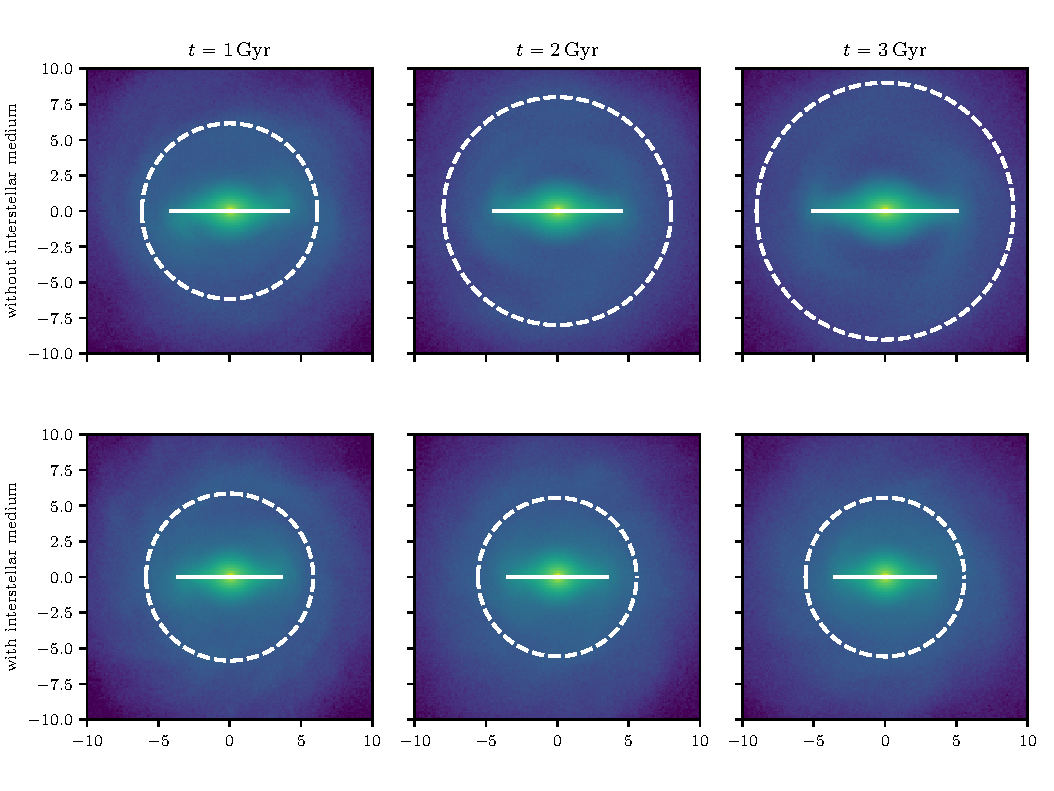
\includegraphics[width=0.8\textwidth]{fig/fig1.pdf}
\caption{Surface density projections in an N-body only simulation (upper
panels) and a simulation which includes the SMUGGLE model (bottom panels). We
can see that in the N-body run, the bar grows in length and strength. In the
SMUGGLE run (which includes a gaseous phase and a model for the multi-phase
interstellar medium), the bar remains at approximately the same length and
strength over the course of the simulation. The N-body model is identical to
the GALAKOS model, discussed in the text.}\label{fig:overview}
\end{figure*}

\begin{figure}[h]%
\centering
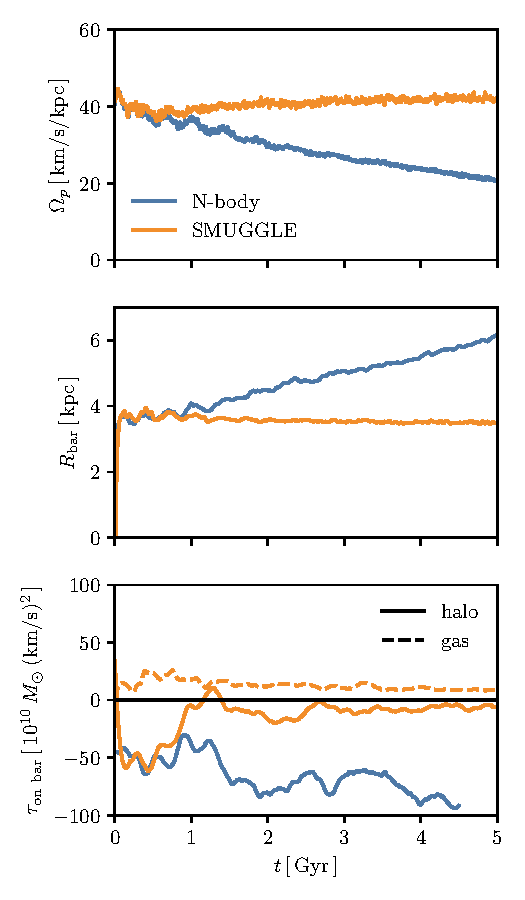
\includegraphics[width=0.45\textwidth]{fig/fig2.pdf}
\caption{Various bar properties from the N-body and SMUGGLE runs. The
\textit{upper panel} show the evolution of the pattern speed. As expected, the
bar in the N-body run slows down due to interactions between the bar and the
dark matter halo. However, the bar in the SMUGGLE run does not slow down and
instead remains at a constant pattern speed. The \textit{middle panel} shows
the evolution of the bar length. In the N-body case, the bar lengthens. This
occurs because as the pattern speed drops, bar-like orbits at larger radii are
possible. Stars are captured on these orbits, lengthening the bar. This
process does not occur in the SMUGGLE cases since the bar pattern speed is not
decreasing, and therefore the bar length remains constant. The \textit{lower
panel} shows the torque on the bar by different components. The solid lines
show the torque exerted by the halo in both the N-body and SMUGGLE cases. The
dashed line shows the torque exerted by the gas phase in the SMUGGLE run
(there is no gas in the N-body run). The first $1.5\,\textrm{Gyr}$ of
evolution of the N-body model is not shown. Details on how these properties
are calculated is given in the Methods section.}\label{fig:prop}
\end{figure}

\begin{figure*}[h]%
\centering
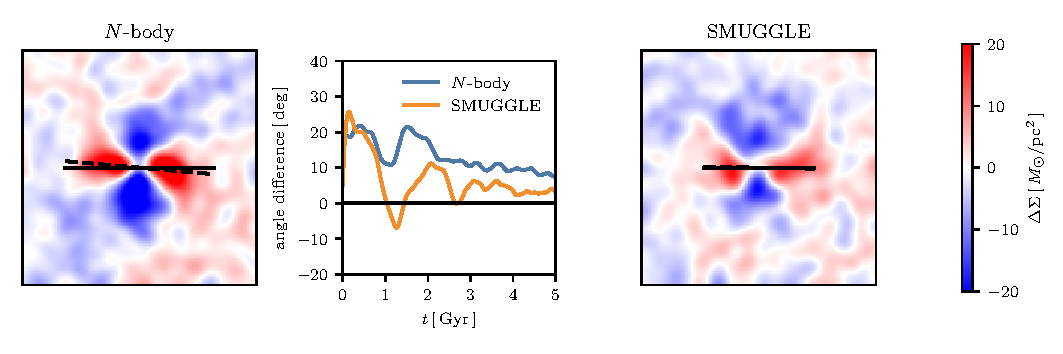
\includegraphics[width=0.9\textwidth]{fig/fig3.pdf}
\caption{The wake excited in the dark matter halo in the N-body case
(\textit{left panel}) and SMUGGLE case (\textit{right panel}) after
$2.6\,\textrm{Gyr}$. The \textit{left} and \textit{right panels} show a
surface density projection in the $x$-$y$ plane of the dark matter halo after
an axisymmetric average has been subracted. The solid line indicates the
direction of the bar while the dashed line indicates the direction of the halo
wake (both measured by taking the second Fourier component within a sphere of
all material within a radius of $X\,\textrm{kpc}$). The \textit{center panel}
shows the time evolution of the angle difference between the bar and the halo
wake, as measured from the second Fourier component. After the first Gyr, the
angle difference in the SMUGGLE case is smaller than in the N-body case by
about a factor of two, reflecting how the dark matter halo in the SMUGGLE case
is unable to exert as negative a torque on the bar as in the N-body
case.}\label{fig:wake}
\end{figure*}

\begin{figure}[h]
\centering
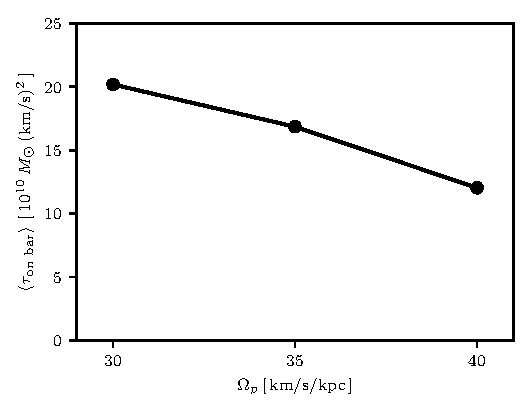
\includegraphics{fig/fig4.pdf}
\caption{The torque on the bar by the gas when the pattern speed of the bar is
kept at a constant value. Only gas within the corotation radius is able to
infall. Since slower bars have larger corotation radii, slower bars experience
a larger net torque than faster bars. The setup of the simulations used here
is identical to the SMUGGLE case discussed earlier and in the Methods section,
except the N-body disk is rotated as a solid body with a constant angular
velocity.}\label{fig:equil}
\end{figure}


%%%%%%%%%%%%%%%%%%%%%%%%%%%%%%%%%%%%%%%%%%%%%%%%%%%%

\bibliography{ref}

\begin{addendum}
  
\item [Acknowledgements] Foo.

\item[Author Contributions] Foo.

  \item[Data Availability] Foo.
    
  \item[Code Availability] Foo.
    
\end{addendum}


%%%%%%%%%%%%%%%%%%%%%%%%%%%%%%%%%%%%%%%%%%%%%%%%%%%%%%%%%%
%%%%%%%%%%%%%%%%%%%%%%%%%%%%%%%%%%%%%%%%%%%%%%%%%%%%%%%%%%

\newpage

\setcounter{page}{1}
\setcounter{figure}{0}
\setcounter{table}{0}
\captionsetup[figure]{labelformat=empty}
\renewcommand{\figurename}{Extended Data Figure}
\renewcommand{\thetable}{Extended Data \arabic{table}}

\begin{center}
{\bf \Large \uppercase{Methods} }
\end{center}

\noindent
{\bf SMUGGLE Model}
\\
\noindent
We use the Stars and MUltiphase Gas in GaLaxiEs (SMUGGLE) model
\cite{2019MNRAS.489.4233M} implemented within the moving-mesh, finite-volume
hydrodynamics code AREPO \cite{2010MNRAS.401..791S}. The SMUGGLE model
includes self-gravity, hydrodynamics, radiative heating and cooling, star
formation, and stellar feedback. Explicit gas cooling and heating of the
multi-phase interstellar medium is implemented, covering temperature ranges
between $10$ and $10^8\,\textrm{K}$.

Star formation occurs in cells above a density threshold
($n_{\textrm{th}}=100\,\textrm{cm}^{-3}$) according to SH03 with a
star-formation efficiency of $\epsilon = 0.01$. Star formation converts gas
cells into star particles which represent single stellar populations. For each
star particle, the deposition of energy, momentum, and mass from stellar winds
and supernovae is modeled. Photoionization and radiation pressure are modeled
using an approximate treatment. A more detailed description of this model can
be found in the flagship SMUGGLE paper.\cite{2019MNRAS.489.4233M}

\vspace{12pt}

\noindent
{\bf Initial Setup}
\\
\noindent
The initial setup of the galactic disk used in this work follows closely the
GALAKOS model\cite{2020ApJ...890..117D}, which uses a modified version of
\texttt{MakeNewDisk}.\cite{2005MNRAS.361..776S} The GALAKOS model has three
components - a radially exponential and vertically isothermal stellar disk,
and a stellar bulge and dark matter halo following a Hernquist
profile.\cite{1990ApJ...356..359H} All N-body runs in this work used the same
setup parameters as the GALAKOS disk, more details of which can be found in
the original paper.

The addition of the gas phase was done as follows. The version of
\texttt{MakeNewDisk} used for the original GALAKOS model can generate a gas
disk which is radially exponential and in vertical gravito-hydrodynamic
balance. We modified the radial profile of this code in order to allow us to
generate a disk with a constant surface density within some cut-off radius,
and then exponentially declining beyond that radius with the scale-length of
the stellar disk. We used an initial surface density of
$20\,M_{\odot}/\textrm{pc}^2$ and a cut-off radius of $9.3\,\text{kpc}$. We
varied the surface density in TEST.

After generating the gaseous disk in this way, we stitched the gas disk
together with the GALAKOS N-body disk (and bulge and dark matter halo) after
the GALAKOS disk has been allowed to evolve for $1.5\,\textrm{Gyr}$. The
purpose of allowing the GALAKOS to evolve first for a short period of time is
to allow for the bar to form unimpacted by the presence of the gas (which
would normally disrupt the formation of the bar). We made one additional
modification when stitching the gas disk together with the N-body disk - we
created a vacuum within the central $4\,\textrm{kpc}$. This vacuum guards
against an initial dramatic infall of gas within the bar region, which we
found to destroy the bar.

Our setup is initially out of equilibrium, but we found that after
$\sim500\,\textrm{Myr}$, the entire system has settled into a steady-state
configuration and initial transients appear not to affect the results after
this point. The constant surface density of the initial gas disk is important
for ensuring the gas disk is dense enough in order for comparisons to real
galaxies to be appropriate. We show the evolution of the surface density
profile in Extended Data Fig.~\ref{fig:surf} compared to observational
estimates (CITE).

\begin{figure}[h]%
\centering
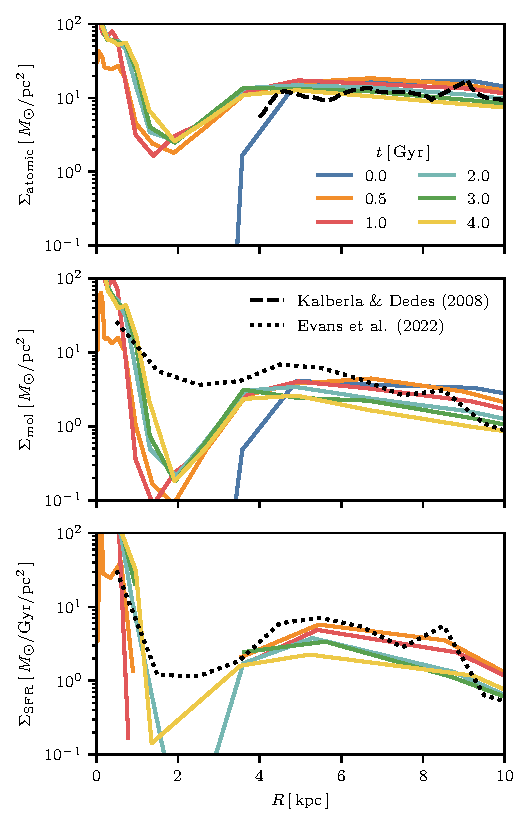
\includegraphics[width=0.45\textwidth]{fig/fig-surf.pdf}
\caption{The time evolution of the gas surface density (\textit{upper}) and the star formation rate (SFR) surface density (\textit{lower}).  } \label{fig:surf}
\end{figure}



\vspace{12pt}

\noindent
{\bf Title}
\\
\noindent
Next section.

% \bibliography{ref2}



\end{document}



